% ------------------------------------------------------------------------------
% LaTeX template created by
% Iker Algañaraz, May Juarez F., Gastón A. Lozano S., Belén N. Paz
% ------------------------------------------------------------------------------

\documentclass[a4paper,12pt]{article}

% ------------------------------------------------------------------------------
% Packages
% ------------------------------------------------------------------------------
\usepackage{anysize} % Márgenes
\usepackage[hypcap=false, font=small, justification=centering, labelfont=bf]{caption} % Pie de foto/tabla
\usepackage{multicol} % Columnas
\usepackage{amsmath} % Fórmulas matemáticas
\usepackage{amssymb} % Símbolos matemáticos
\usepackage{amsfonts} % Font matemática
\usepackage[utf8]{inputenc} % Facilitar la escritura en español
\usepackage{xcolor} % Color del texto
\usepackage{graphicx} % Figuras
\usepackage[spanish,es-tabla]{babel} % Tipografía del idioma
\usepackage{booktabs} % Separación en tablas
\usepackage{multirow} % Multirow en tablas
\usepackage{hyperref} % Refs como hyperlinks
\usepackage{subfig}
\usepackage{subcaption}
%\usepackage{biblatex} % Bibliografía automática a partir de base bib

%\usepackage{array}
%\usepackage{verbatim} % Comentarios multilinea
%\usepackage{siunitx} % Unidades del sistema internacional
%\usepackage{fancyhdr} % Personalizar encabezado y pie de pagina
%\usepackage{longtable} % Tablas largas
%\usepackage{blindtext} % Lore ipsum
%\usepackage{soul} % Subrayar
%\usepackage{grffile}
%\usepackage{mathrsfs}

% ------------------------------------------------------------------------------
% Config
% ------------------------------------------------------------------------------
\newenvironment{Figure}
    {\par\medskip\noindent\minipage{\linewidth}}
    {\endminipage\par\medskip}

\providecommand{\keywords}[1] % Keywords
{
    \small	
    \textbf{\textit{Keywords---}} #1
}

\providecommand{\abs}[1]{\lvert#1\rvert} % Valor absoluto

\renewcommand{\thefootnote}{\Roman{footnote}}

\marginsize{2cm}{2cm}{1cm}{2cm} % pkg: anysize

\graphicspath{{./Fotos/}} % pkg: graphicx

\setlength\columnsep{18pt}
\setlength\parskip{4pt} \setlength\parindent{0in}

\title{Propulsion using linear induction motors\\ 
\medskip \large Universidad Nacional de Tucumán}
\author{May Juarez Ferriol}
\date{}

% ------------------------------------------------------------------------------
% Document
% ------------------------------------------------------------------------------
\begin{document}

\begin{titlepage}

    \begin{center}

        \vspace*{2cm}

        \Huge
        Estudio de fuerzas ferromagnéticas \\
        usando un motor de solenoide

        \vspace{1cm}

        \LARGE
        Juarez Ferriol May

        \vspace{1cm}

        
\includegraphics[width=0.35\textwidth]{unt.jpg}

        \vspace{1cm}

        \Large
        Licenciatura en Física

        Facultad de Ciencias Exactas y Tecnología

        Universidad Nacional de Tucumán

        Tucumán, Argentina

        \vspace{1cm}

        Diciembre 2023

        \vspace{1cm}

        Supervisor: Prof. Leal Sebastián

    \end{center}

\end{titlepage}

\section*{Resumen}

    

\section*{Introducción}

    Como sabemos de los efectos magnéticos encontrados día a día, cuando acercamos un imán permanente o un electroimán a un elemento ferromagnético, éste se ve atraído a éste. ¿Pero con qué fuerza es atraído?

    El conocimiento técnico requerido para responder esta pregunta es mayor al que se suele tener cuando se ve por primera vez el tema de magnetismo, así que los libros generales de física no suelen incluir su respuesta. 
    
    Vimos que se analizan fuerzas magnéticas entre dos materiales que cada uno genera campo magnético. Este informe busca explicar de manera sencilla y concisa cómo podemos estimar esta fuerza entre un generador de campo magnético y un elemento ferromagnético, y usarla para distintas aplicaciones, como un motor rotatorio de solenoide, usado para muchísimas aplicaciones a lo largo del mundo, o motores lineales sincrónicos, que son los usados en los portaaviones para la propulsión de aviones, o en el tren bala de Japón para su movimiento.

\section*{Marco teórico}

    \subsection*{Campos magnéticos en solenoides}

    \subsubsection*{Campo magnético de un solenoide infinito en el vacío\footnote{Cuando hablamos de algo infinito en el campo de la física, nos estamos refiriendo a valores relativos. En este caso consideramos infinito cuando el largo del solenoide es mucho mayor que el diámetro de éste.}}

        Un solenoide es cualquier dispositivo físico capaz de crear un campo magnético sumamente uniforme e intenso en su interior, y muy débil en el exterior. Un ejemplo teórico es el de una bobina de hilo conductor aislado y enrollado helicoidalmente, de longitud infinita. En ese caso ideal el campo magnético sería uniforme en su interior y fuera sería nulo.

        En la práctica, una aproximación real a un solenoide es un alambre aislado, de longitud finita, enrollado en forma de hélice (bobina), por el que circula una corriente eléctrica. Cuando esto sucede, se genera un campo magnético dentro de la bobina tanto más uniforme cuanto más larga sea la bobina.

        \begin{Figure}
            \centering

            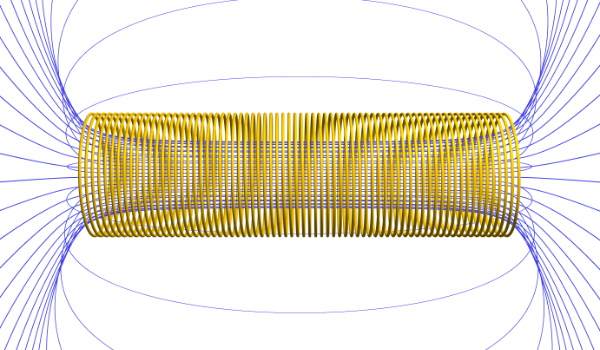
\includegraphics[width=0.6\linewidth]{Solenoide.jpg}
            \label{fig: solenoide}
            \captionof{figure}{Solenoide en el que circula corriente. Las líneas azules representan el campo magnético}
        \end{Figure}

        En el caso de un solenoide infinito en el vacío, se puede obtener el módulo del campo magnético en el eje axial con la ecuación (\ref{eq: campoMagneticoSolenoideInfinito}), donde $\mu_0$ es la constante de permeabilidad magnética en el vacío, N el número de espiras del solenoide, I la corriente que circula, y L la longitud total del solenoide.

        \begin{equation}
            \label{eq: campoMagneticoSolenoideInfinito}
            B_x = \frac{\mu_0 N I}{L}
        \end{equation}

    \subsubsection*{Campo magnético de un solenoide finito en el vacío}
    
        En el caso de un solenoide finito, con x = 0 siendo el centro del solenoide, y estando en el vacío, podemos calcular el campo magnético en el eje axial con la ecuación (\ref{eq: campoMagneticoSolenoideFinito}).

        \begin{equation}
            \label{eq: campoMagneticoSolenoideFinito}
            B_x = \frac{\mu_0 N I}{2L} \left[ \frac{L/2 - x}{\sqrt{(L/2 - x)^2 + r^2}} + \frac{L/2 + x}{\sqrt{(L/2 + x)^2 + r^2}} \right]
        \end{equation}

    \subsubsection*{Campo magnético de un solenoide con un núcleo ferromagnético}

        Las ecuaciones que hemos discutido hasta ahora son válidas para solenoides en el vacío, lo que significa que la permeabilidad del campo magnético es la misma que la del vacío, $\mu_0$.

        Si el solenoide está inmerso en un material con permeabilidad relativa $\mu_r$, entonces el campo se incrementa proporcionalmente a esa cantidad, que podemos ver modificando la ecuación (\ref{eq: campoMagneticoSolenoideInfinito}), obteniendo la ecuación (\ref{eq: campoMagneticoSolenoideInfinitoRelativo}).

        \begin{equation}
            \label{eq: campoMagneticoSolenoideInfinitoRelativo}
            B_x = \frac{\mu_r\mu_0 N I}{L}
        \end{equation}

        En la mayoría de los solenoides, éste no se encuentra sumergido en un material de mayor permeabilidad, si no que parte del espacio alrededor del solenoide tiene el material de mayor permeabilidad, y parte del espacio alrededor es simplemente aire, que se comporta muy parecido al vacío. En ese caso, el efecto completo del material de mayor permeabilidad no se ve, si no que va a existir una permabilidad efectiva, o aparente, $\mu_{ef}$ de manera que $1 \leq \mu_{ef} \leq \mu_r$.

        La inclusión de un nucleo ferromagnético aumenta la permeabilidad efectiva del campo magnético, como se puede ver para un solenoide infinito en la ecuación (\ref{eq: campoMagneticoSolenoideInfinitoEfectivo}).

        \begin{equation}
            \label{eq: campoMagneticoSolenoideInfinitoEfectivo}
            B_x = \frac{\mu_{ef}\mu_0 N I}{L}
        \end{equation}

    \subsubsection*{Campo magnético de un solenoide finito con un núcleo ferromagnético}

        Si juntamos lo discutido anteriormente sobre el solenoide finito y el núcleo ferromagnético, llegamos a la ecuación (\ref{eq: campoMagneticoSolenoideFinitoEfectivo}).

        \begin{equation}
            \label{eq: campoMagneticoSolenoideFinitoEfectivo}
            B_x = \frac{\mu_{ef}\mu_0 N I}{2L} \left[ \frac{L/2 - x}{\sqrt{(L/2 - x)^2 + r^2}} + \frac{L/2 + x}{\sqrt{(L/2 + x)^2 + r^2}} \right]
        \end{equation}

        En los extremos del solenoide (obtención de la ecuación en el apéndice A), el campo magnético es igual a la ecuación (\ref{eq: campoMagneticoSolenoideFinitoEfectivoExtremos}).

        \begin{equation}
            \label{eq: campoMagneticoSolenoideFinitoEfectivoExtremos}
            B_x = \frac{\mu_{ef}\mu_0 N I}{2\sqrt{L^2 + r^2}}
        \end{equation}

        Como se esperaría de un sistema en donde la dirección negativa y positiva es arbitraria y no modifica nada, los campos magnéticos son simétricos respecto al punto central del solenoide.

    \subsection*{Elementos magnéticos}

        Los átomos que forman a toda la materia contienen electrones en movimiento, los cuáles forman espiras microscópicas de corriente que producen campos magnéticos. En muchos materiales, estas corrientes están orientadas al azar, y no generan un campo magnético neto. Sin embargo, en algunos materiales, un campo magnético externo puede causar que estas espiras se orienten de forma preferencial con el campo, de manera que sus campos magnéticos se sumen al campo exterior. En ese caso decimos que el material se ha magnetizado. 

        En base a los orígenes atómicos de las propiedades magnéticas de un material, podemos discutir tres clases generales de comportamientos magnéticos, \emph{paramagnetismo}, \emph{diamagnetismo}, y \emph{ferromagnétismo}. 

        El paramagnetismo y el diamagnetismo están fuera del alcance de este informe, pero en síntesis, el paramagnetismo tiene un momento magnético total $\mu_b$ que al colocarse en un campo magnético externo, éste ejerce una torca sobre cada momento magnético, de acuerdo con la ecuación $\vec{\tau} = \vec{\mu} \times \vec{B}$. Estas torcas tienden a alinear los momentos magnéticos con el campo, donde en esa posición las direcciones de las espiras de corriente son tales que se suman al campo magnético externo. El campo magnético en cualquier punto del material es mayor por un factor $\mu_r$, que para sólidos y líquidos paramagnéticos comunes, suele variar entre 1.00001 a 1.003, es decir, muy poca variación respecto a 1, además de que disminuye cuando aumenta la temperatura, al aumentar el movimiento térmico aleatorio, el cual tiende a distribuir sus orientaciones al azar.

        El diamagnetismo es el material en el que ante la presencia de campos magnéticos externos, altera los movimientos de los electrones dentro de los átomos, generando espiras de corriente adicionales y dipolos magnéticos inducidos cuya dirección del campo magnético adicional provocados por éstos es siempre opuesta a la dirección del campo externo. Por lo tanto, la permeabilidad relativa es siempre ligeramente menor que 1, comúnmente del orden 0.999990 a 0.99999. Este valor es casi independiente de la temperatura.

    \subsubsection*{Ferromagnetismo}

        En los materiales ferromagnéticos, las interacciones fuertes entre los momentos magnéticos atómicos los llevan a alinearse paralelamente entre sí, en regiones llamadas \emph{dominios magnéticos}, aún cuando no están en presencia de un campo magnético externo. Dentro de cada dominio, casi todos los momentos magnéticos atómicos son paralelos.

        \begin{Figure}
            \centering
            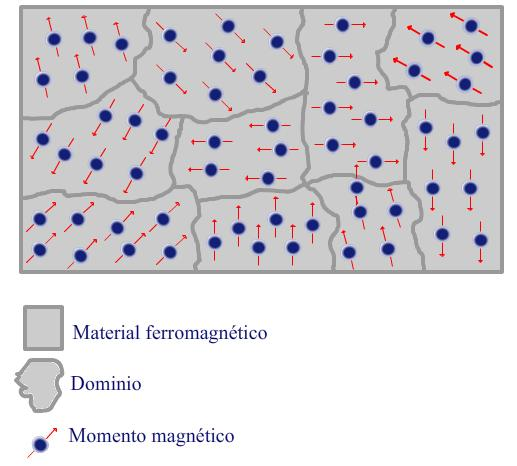
\includegraphics[width=0.4\linewidth]{ferromagnetismo_dominios.jpg}
            \captionof{figure}{Dominios magnéticos en un material ferromagnético}
            \label{fig: ferromagnetismo_dominios}
        \end{Figure}

        Cuando no hay un campo magnético externo aplicado, las magnetizaciones de los dominios están orientadas al azar, pero cuando se aplica un campo externo $\vec{B_0}$, los dominios tienden a ordenarse paralelos al campo. Las fronteras de los dominios también tienden a desplazarse; los dominios magnetizados en dirección del campo crecen, y aquellos que están en otras direcciones disminuyen. La permeabilidad relativa $mu_r$ de los materiales ferromagnéticos es mucho mayor a la unidad, típicamente del rango de 1.000 a 100.000. Por lo tanto, un material ferromagnético como el hierro es fuertemente magnetizado por el campo de un imán permanente o electroimán y es atraído por éste.
        
        \begin{Figure}
            \centering
            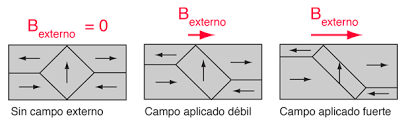
\includegraphics[width=0.6\linewidth]{ferromagnetismo_campoMagneticoAplicado.png}
            \captionof{figure}{Dominios magnéticos en un material ferromagnético con un campo magnético externo aplicado}
            \label{fig: ferromagnetismo_campoMagneticoAplicado}
        \end{Figure}

    \subsection*{Magnetización}

        El campo adicional $\vec{B}$ producido por espiras de corriente microscópicas de los electrones, es proporcional al momento magnético total $\vec{\mu}$ por unidad de volumen V en el material. Esta cantidad vectorial recibe el nombre de magnetización del material.

        \begin{equation}
            \label{eq: magnetizacion}
            \vec{M} = \frac{\vec{\mu_{total}}}{V}
        \end{equation}

        El campo magnético adicional debido a la magnetización del material es igual a $\mu_0 \vec{M}$. Cuando un material de este tipo rodea por completo a un conductor portador de corriente, el campo magnético del material está dado por la ecuación (\ref{eq: campoMagneticoTotal}), donde $\vec{B_0}$ es el campo generado por la corriente en el conductor.

        \begin{equation}
            \label{eq: campoMagneticoTotal}
            \vec{B} = \vec{B_0} + \mu_0 \vec{M}
        \end{equation}

    \subsection*{Fuerza causada por un campo magnético externo a un elemento ferromagnético}

        Una magnetización M dentro de un volumen V encerrado por una superficie S es equivalente a una densidad volumétrica de corriente $J_m = \nabla \times M$ y una densidad superficial de corriente $(M \times n)$. En la ausencia de corrientes macroscópicas, la fuerza magnética total en el cuerpo se puede calcular con la ecuación (\ref{eq: fuerzaMagnetica}).

        \begin{equation}
            \label{eq: fuerzaMagnetica}
            F = - \int_{V}^{} (\nabla \cdot M) B_e \ d^3 x + \int_{S}^{} (M \cdot n) B_e \ da
        \end{equation}

        $B_e$ es la inducción magnética aplicada, sin contar la propia. Si la distribución de la magnetización no es discontinua, la superficie se puede considerar en el infinito, y la fuerza se puede calcular únicamente con la integral de volumen.

        \begin{equation}
            \label{eq: fuerzaMagneticaReducida}
            F = - \int_{V}^{} (\nabla \cdot M) B_e \ d^3 x
        \end{equation}

\section*{Materiales, métodos y recolección de datos}

    \subsection*{Motor de solenoide}

        El motor de solenoide fue creado por Darío Edgardo Ponzetti y donado a la facultad.

        Su funcionamiento se basa en un circuito de corriente continua, constituido por una fuente de tensión variable de 1.5 V a 12 V conectada en serie a un solenoide corto, de alambre esmaltado de cobre de 0.6 mm de diámetro. Dicha conexión permite la generación de un campo magnético intenso en el eje de la bobina, originando el desplazamiento de un pistón (núcleo ferromagnético) ubicado coaxialmente dentro de la misma. El resto del equipo consta de un sistema de transmisión que imprime movimiento de rotación durante medio ciclo a un eje conformado tambien por un volante de inercia el cual entregará torque en el restante semiciclo, razón por la cual se incluye al sistema una leva que accionará la bobina y la desconectara mediante un switch “final de carrera”.

        \begin{Figure}
            \centering

            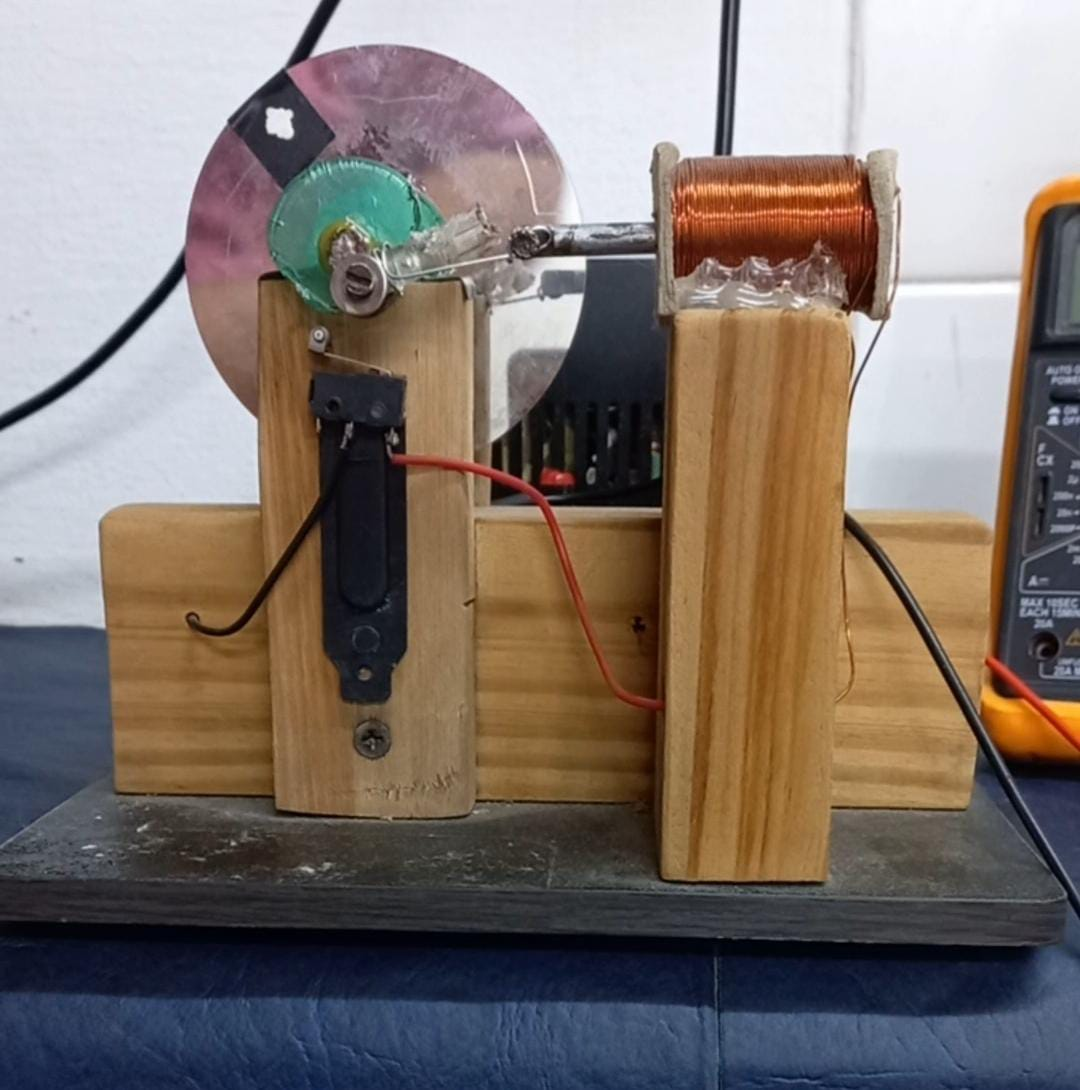
\includegraphics[width=0.4\linewidth]{motorSolenoide_frente.jpg}
            \label{fig: motorSolenoide_frente}
                
            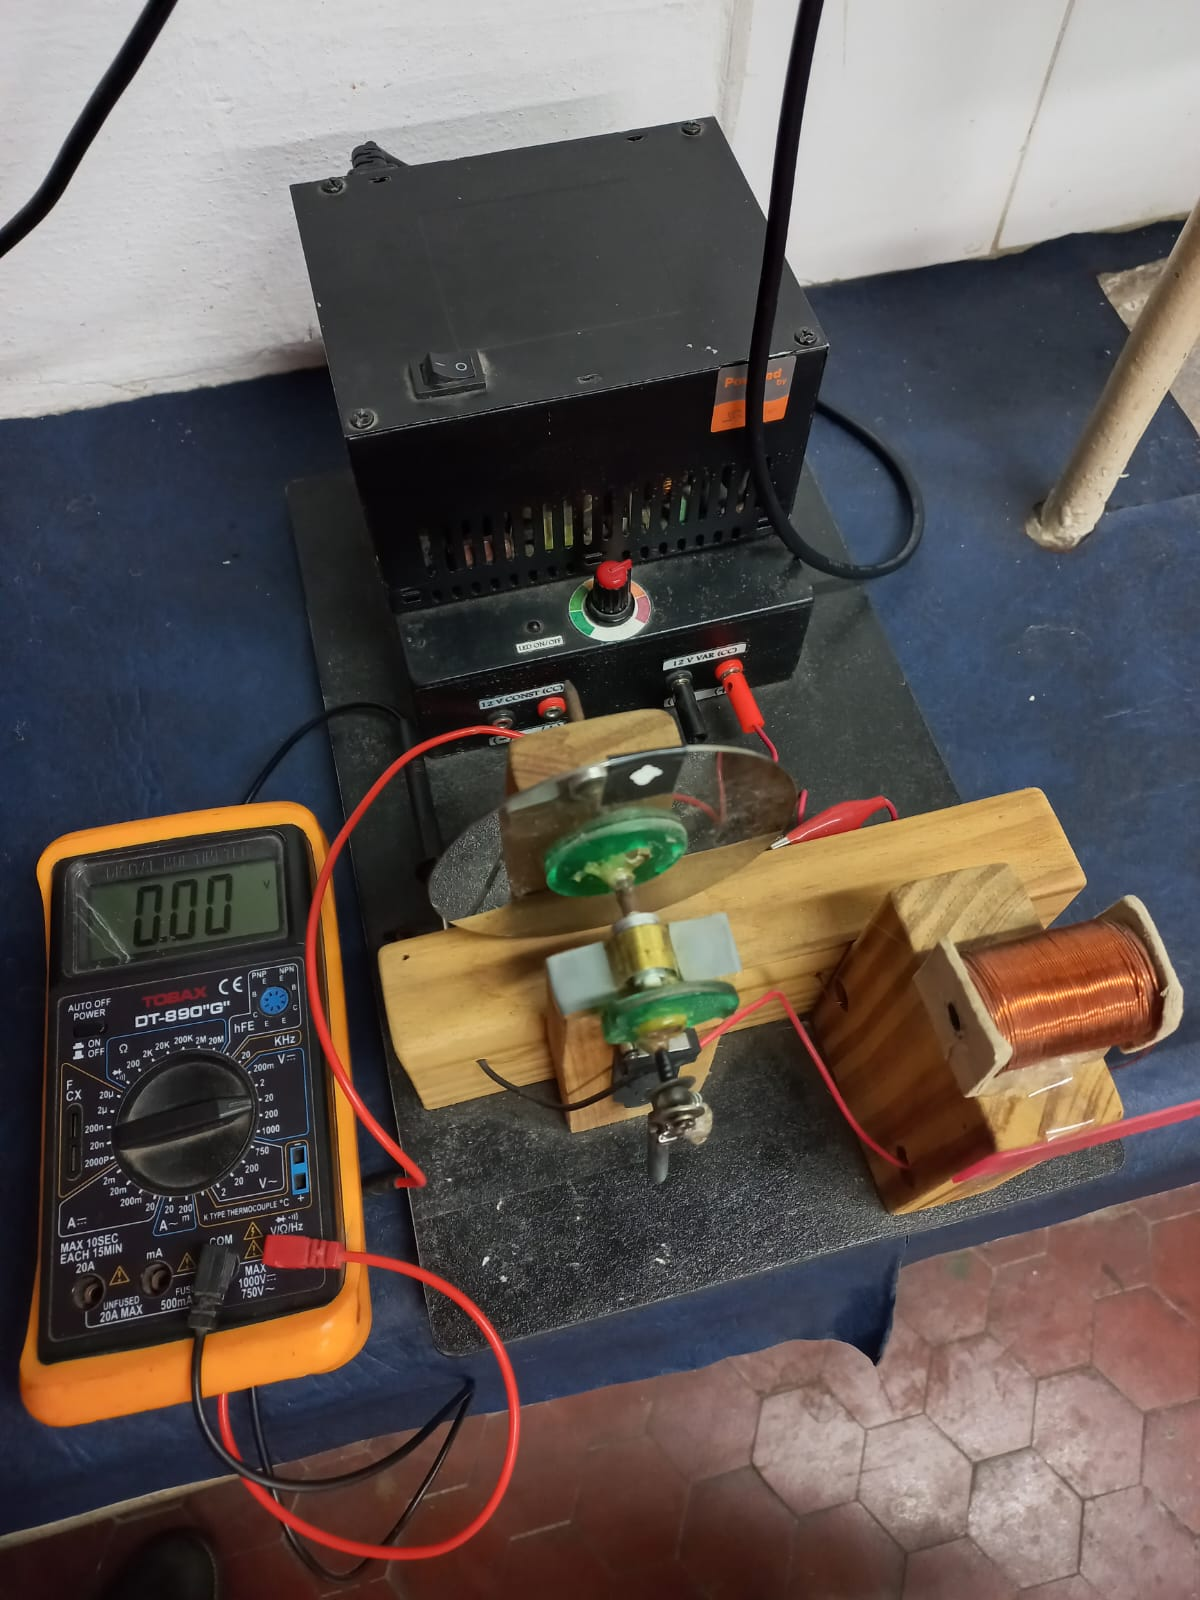
\includegraphics[width=0.4\linewidth]{motorSolenoide_superior.jpg}
            \label{fig: motorSolenoide_superior}

            \captionof{figure}{Motor solenoide}

        \end{Figure}

    \subsection*{Métodos}

        Utilizando el motor de solenoide, y un voltímetro, se fue variando la tensión proporcionada por la fuente de corriente continua, y se graficó el movimiento lineal del pistón usando Tracker, el cual tiene el mismo período que el movimiento angular del disco de inercia.

        \begin{Figure}
            \centering

            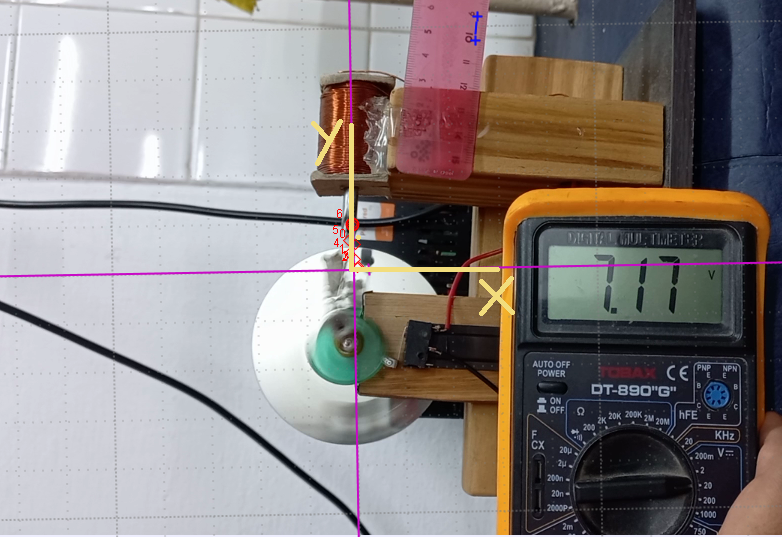
\includegraphics[width=0.5\linewidth]{mediciones_movimientoLinealCoordenadas.png}
            \label{fig: mediciones_movimientoLinealCoordenadas}
            \captionof{figure}{Sistema de coordenadas para la gráfica de movimiento lineal del pistón}
        \end{Figure}


        \begin{Figure}
            \centering

            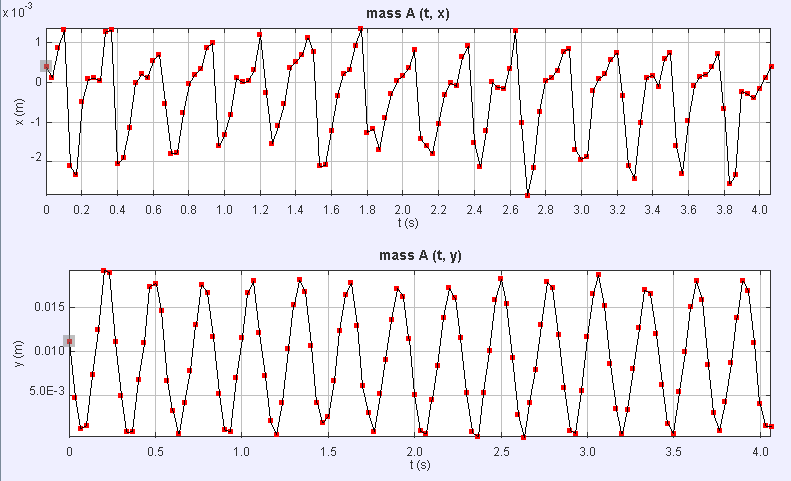
\includegraphics[width=0.6\linewidth]{mediciones_movimientoLineal.png}
            \label{fig: mediciones_movimientoLineal}
            \captionof{figure}{Gráfica de movimiento lineal del pistón para un valor de 7 V}
        \end{Figure}

        No nos interesan los valores de movimiento que se encuentren en el eje de las abcisas, ya que estamos ante el supuesto de que el movimiento es coaxial al solenoide.

        Con estos datos medidos, se calculó numéricamente la segunda derivada y se obtuvo la aceleración en función del tiempo (Fig. \ref{fig: mediciones_aceleracion}).

        \begin{Figure}
            \centering

            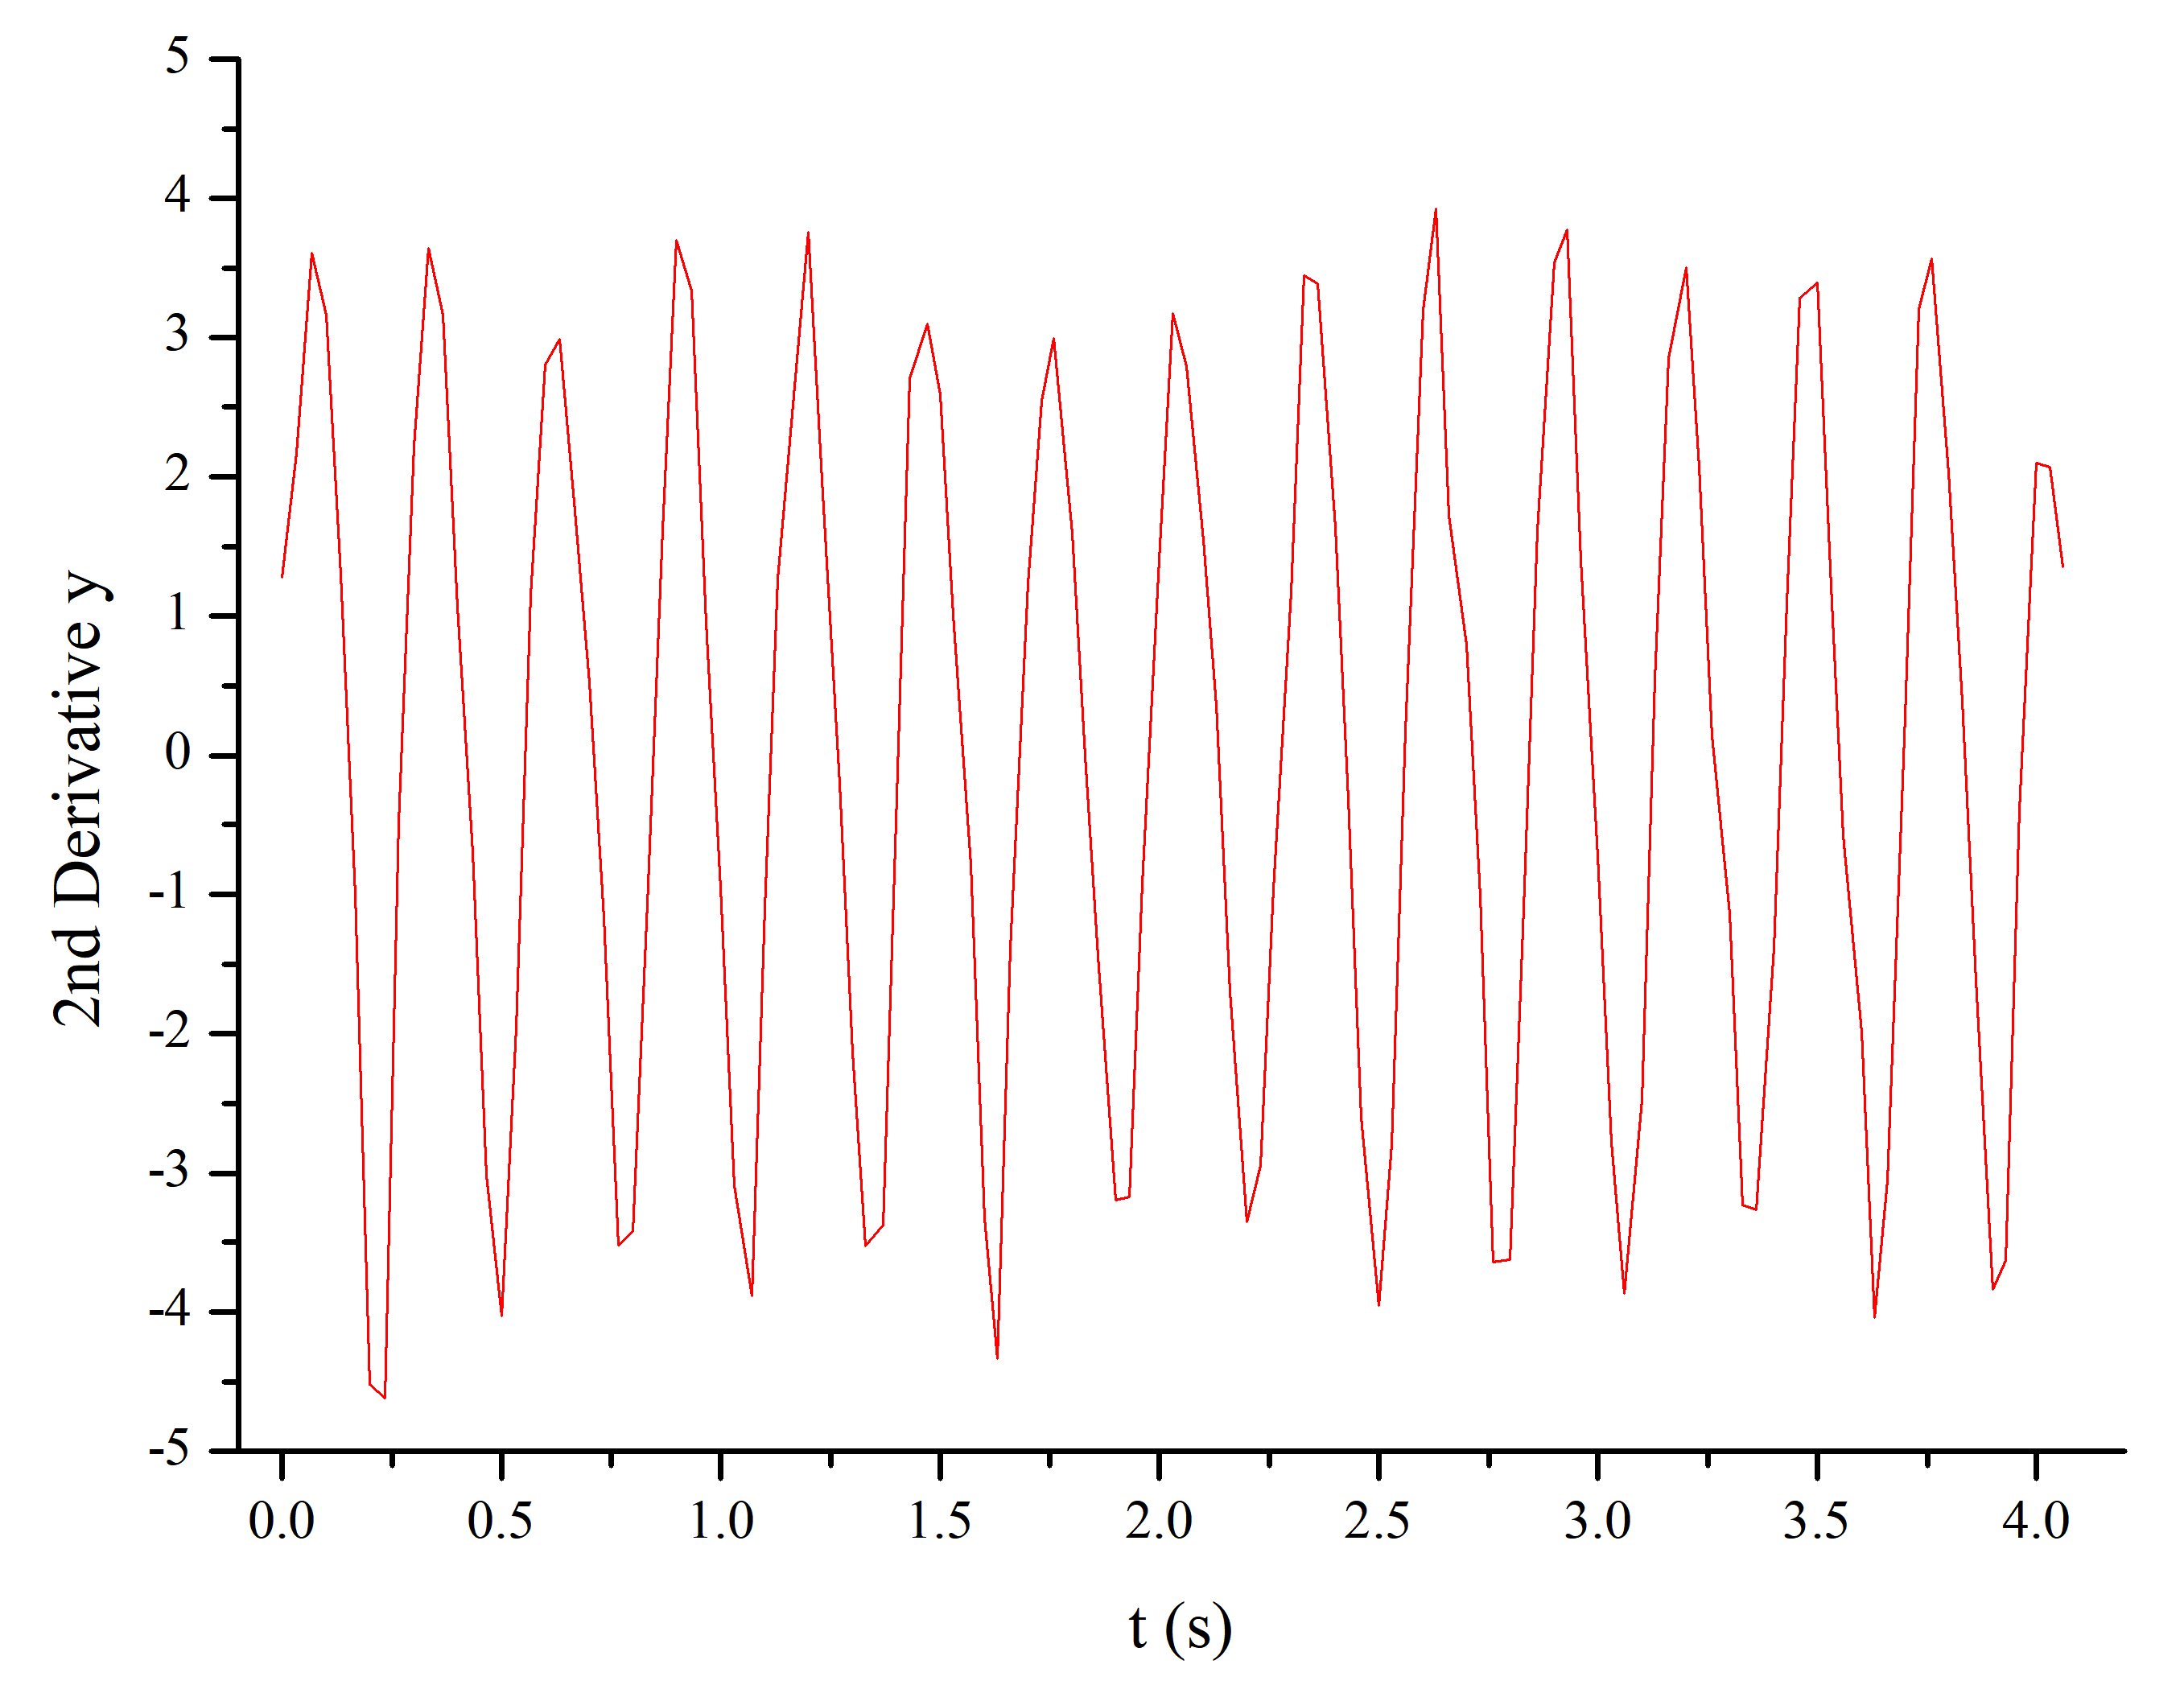
\includegraphics[width=0.6\linewidth]{mediciones_aceleracion.png}
            \label{fig: mediciones_aceleracion}
            \captionof{figure}{Gráfica de movimiento lineal del pistón para un valor de 7 V al inicio de su movimiento}
        \end{Figure}

\section*{Resultados}

    

\section*{Conclusión y discusiones}

    \subsection*{Recapitulación de los objetivos}



    \subsection*{Resumen e implicación de los resultados}



    \subsection*{Futuras investigaciones}

        

\section*{Agradecimientos}

    

\section*{Apéndice A - Campo magnético en los extremos del \\solenoide}

Empezando por la ecuación de campo magnético de un solenoide finito con un núcleo ferromagnético (\ref{eq: campoMagneticoSolenoideFinitoEfectivo}).

    \begin{equation*}
        B_x = \frac{\mu_{ef}\mu_0 N I}{2L} \left[ \frac{L/2 - x}{\sqrt{(L/2 - x)^2 + r^2}} + \frac{L/2 + x}{\sqrt{(L/2 + x)^2 + r^2}} \right]
    \end{equation*}

    En el extremo izquierdo ($x=-L/2$)

    \begin{equation*}
        B_x = \frac{\mu_{ef}\mu_0 N I}{2L} \left[ \frac{L/2 - (-L/2)}{\sqrt{(L/2 - (-L/2))^2 + r^2}} + \frac{L/2 + (-L/2)}{\sqrt{(L/2 + (-L/2))^2 + r^2}} \right]
    \end{equation*}

    \begin{equation*}
        B_x = \frac{\mu_{ef}\mu_0 N I}{2L} \left[ \frac{L/2 + L/2}{\sqrt{(L/2 + L/2)^2 + r^2}} + \frac{L/2 - L/2}{\sqrt{(L/2 - L/2)^2 + r^2}} \right]
    \end{equation*}

    \begin{equation*}
        B_x = \frac{\mu_{ef}\mu_0 N I}{2L} \left[ \frac{L}{\sqrt{L^2 + r^2}} \right]
    \end{equation*}

    \begin{equation*}
        B_x = \frac{\mu_{ef}\mu_0 N I}{2\sqrt{L^2 + r^2}}
    \end{equation*}

De manera análoga en el extremo derecho ($x=L/2$)

    \begin{equation*}
        B_x = \frac{\mu_{ef}\mu_0 N I}{2L} \left[ \frac{L/2 - (L/2)}{\sqrt{(L/2 - (L/2))^2 + r^2}} + \frac{L/2 + (L/2)}{\sqrt{(L/2 + (L/2))^2 + r^2}} \right]
    \end{equation*}

    \begin{equation*}
        B_x = \frac{\mu_{ef}\mu_0 N I}{2L} \left[ \frac{L/2 - L/2}{\sqrt{(L/2 - L/2)^2 + r^2}} + \frac{L/2 + L/2}{\sqrt{(L/2 + L/2)^2 + r^2}} \right]
    \end{equation*}

    \begin{equation*}
        B_x = \frac{\mu_{ef}\mu_0 N I}{2L} \left[ \frac{L}{\sqrt{L^2 + r^2}} \right]
    \end{equation*}
    
    \begin{equation*}
        B_x = \frac{\mu_{ef}\mu_0 N I}{2\sqrt{L^2 + r^2}}
    \end{equation*}

\begin{thebibliography}{99}

    \bibitem{} D. E. Ponzetti, \emph{Proyecto experimental: Motor solenoide.} (Tucumán, 2018)

    \bibitem{} H. D. Young, R. A. Freedman, \emph{Sears and Zemansky's University Physics: with Modern Physics}, 14th ed. (Pearson, San Francisco, 2015).

\end{thebibliography}


\end{document}

% ------------------------------------------------------------------------------
% Common references and examples
% ------------------------------------------------------------------------------
% 
% ---------------------------
% Bibliography
% ---------------------------
% \bibitem{} Sears, Zemansky. \emph{Física universitaria}, vol. 2, 14th ed. Pearson Education, 2018.
% \bibitem{} Hecht, Zajac. \emph{Óptica}, 4th ed. Pearson Education, 2003.
% \bibitem{} Serway, Jewett. \emph{Physics for Scientists and Engineers}, vol. 2, 6th ed. Brooks Cole, 2004.
% \bibitem{} Jenkins, White. \emph{Fundamentos de óptica}, 3th ed. Aguilar S.A., 1964.
%
% ---------------------------
% Tables
% ---------------------------
% \begin{Figure}
%     \centering
%
%     \begin{tabular}{c|c}
%         \toprule
%          & \textit{...} \\
%          & \textit{[]} \\
%         \midrule
%         ... & \multirow{2}{*}{$(... \pm ...)$} \\
%         ... & \\
%         ... & \multirow{2}{*}{$(... \pm ...)$} \\
%         ... & \\ \hline
%         ... & $(... \pm ...)$ \\
%         ... & $(... \pm ...)$ \\
%         \bottomrule
%     \end{tabular}
%
%     \captionof{table}{}
%     \label{tab:}
% \end{Figure}
%
% \begin{Figure}
%     \centering
%
%     \begin{tabular}{cc}
%         \toprule
%         \textit{\textbf{... []}} & \textit{\textbf{$... []}}\\
%         \midrule
%         $... \pm ...$ & $... \pm ...$ \\
%         $... \pm ...$ & $... \pm ...$ \\
%         \bottomrule
%     \end{tabular}
%
%     \captionof{table}{}
%     \label{tab:}
% \end{Figure}
%
% ---------------------------
% Figures
% ---------------------------
% \begin{Figure}
%     \centering
%     \includegraphics[width=1\linewidth]{.jpg}
%     \captionof{figure}{}
%     \label{fig:}
% \end{Figure}
%
% ---------------------------
% Equations
% ---------------------------
% \begin{equation}
%     \label{eq:}
%     ...
% \end{equation}